%\documentclass[handout]{beamer}
\documentclass{beamer}

\usepackage{amsmath,amsfonts,amssymb,graphicx} 
\usefonttheme[onlymath]{serif}
% use article-like math letters, from http://tex.stackexchange.com/questions/34265/how-to-get-beamer-math-to-look-like-article-math


\newcommand\bi{\begin{itemize}}
\newcommand\ei{\end{itemize}}
\newcommand\simMC{\stackrel{\scriptscriptstyle{MC}}{\sim}}


% from genPomp ms
\newcommand\T{\mathbb{T}}
\newcommand\transmission{\mathcal{T}}
\newcommand\observation{\mathcal{G}}
\newcommand\observationTree{genetic tree}
\newcommand\descendents{h}
\newcommand\sequenceLabel{q}
\newcommand\tInit{t_{0}}
\newcommand\tRoot{t_{\mathrm{root}}}
\newcommand\tEnd{t_{\mathrm{end}}}
\newcommand{\circled}[1]{
  \kern-0.4em \raisebox{.1pt}{\textcircled{\raisebox{-.9pt} {#1}}}
}

\usepackage{natbib}
\usepackage{url}
%\usepackage{ulem}
%\renewcommand\emph[1]{{\it #1}} % the ulem package redefines \emph
%\renewcommand\em{\it} % the ulem package redefines \emph

\usepackage{xcolor}
\usepackage{colortbl}
%\definecolor{olive}{rgb}{0.3, 0.4, .1}
%\definecolor{dgreen}{rgb}{0.,0.6,0.}
%\definecolor{gold}{rgb}{1.,0.84,0.}
%\definecolor{JungleGreen}{cmyk}{0.99,0,0.52,0}
%\definecolor{BlueGreen}{cmyk}{0.85,0,0.33,0}
%\definecolor{RawSienna}{cmyk}{0,0.72,1,0.45}
%\definecolor{Magenta}{cmyk}{0,1,0,0}

\usepackage{graphicx} % Allows including images
%\usepackage{booktabs} % Allows the use of \toprule, \midrule and \bottomrule in tables
\mode<presentation> {

\usetheme{Madrid}

%%\setbeamertemplate{footline}[frame number]
\setbeamertemplate{footline}{
  \hfill%
  \usebeamercolor[fg]{page number in head/foot}%
  \usebeamerfont{page number in head/foot}%
  \setbeamertemplate{page number in head/foot}[framenumber]%
  \usebeamertemplate*{page number in head/foot}\kern1em\vskip2pt%
}

\setbeamertemplate{navigation symbols}{} 

}

\newcommand\myemph[1]{{\textbf{#1}}}
\newcommand\enumerateSpace{\hspace{2mm}}
\usepackage{amssymb}
\newenvironment {myitemize} {
                 \begin{list}{\textcolor{black}{$\bullet$} \hfill}
%                 \begin{list}{\textcolor{blue}{{\small{$\blacktriangleright$}}} \hfill}
                 {\setlength{\labelwidth}{0.3 cm}
                  %\setlength{\leftmargin}{0em}
                  \setlength{\leftmargin}{0.15cm}
                  \setlength{\itemindent}{0.15cm}
                  \setlength{\labelsep}{0cm}
                  \setlength{\parsep}{0.2 ex}
%                  \setlength{\itemsep}{0.25 cm}
                  \setlength{\itemsep}{1 mm}
%                   \setlength{\itemsep}{0.0 cm}
      \setlength{\topsep}{0.0cm}}} %space between title and 1st item
   {\end{list}}

\newcommand\code[1]{\texttt{#1}}
\usepackage{url}

%% customized math macros
\newcommand\prob{\mathbb{P}}
\newcommand\E{\mathbb{E}}
\newcommand\dd[1]{\mathrm{d}{#1}}
\newcommand\given{{\,\vert\,}}
\newcommand\equals{{{\,}={\,}}} 
\newcommand\myequals{\hspace{0.5mm}{=}\hspace{0.5mm}}
\newcommand\myto{{\;:\;}}
\newcommand\seq[2]{{#1}\!:\!{#2}}
\newcommand\mydot{{\,\cdot\,}}
\newcommand\cp[2]{N_{\mathrm{#1}\mathrm{#2}}}
\newcommand\giventh{{\hspace{0.5mm};\hspace{0.5mm}}}
%\newcommand\normal{{\mathrm{Normal}}}
\newcommand\normal{\mathcal{N}}
\newcommand\argequals{{\,=\,}}
\newcommand\lags{c}
\newcommand\maxlag{\overline{c}}
\newcommand\nlfList{C}
\newcommand\bigO{\mathcal{O}}
\newcommand\loglik{\lambda}
\newcommand\loglikMC{\MC{\loglik}}
\newcommand\R{\mathbb{R}}
\newcommand\param{\,;}
\newcommand\mycolon{{\hspace{0.6mm}:\hspace{0.6mm}}}
\newcommand\MC[1]{#1^{\,\mbox{\tiny MC}}}
%\newcommand\EMC{\MC{\E}}
\newcommand\EMC{{\E}}
\newcommand\Var{\mathrm{Var}}
\newcommand\var{\Var}
\newcommand\Cov{\mathrm{Cov}} 
\newcommand\cov{\Cov}
\newcommand\iid{\mathrm{iid}}
%\newcommand\dist{\mathrm{dist}}
\newcommand\dist{d}
\newcommand\transpose{\top}

%% for particle filters
\newcommand\unit{u}
\newcommand\altUnit{\tilde u}
\newcommand\Unit{U}
%\usepackage[mathscr]{euscript}
\renewcommand\time{n}
%\renewcommand\vec[1]{\boldsymbol{#1}}
\newcommand\Time{N}
\newcommand\Np{J}
\newcommand\np{j}


%% for flow diagrams
\usepackage{tikz}
\usetikzlibrary{positioning}
\usetikzlibrary {arrows.meta}
\usetikzlibrary{shapes.geometric}

\begin{document}

\begin{frame}
  
\begin{center}
  {\Large\bf Inference on spatiotemporal infectious disease dynamics}

%ABSTRACT: Epidemiological models must be consistent with observed data in order to generate reliable knowledge and evidence-based policy. Metapopulation systems, which consist of a network of connected sub-populations, pose technical challenges in statistical inference owing to nonlinear, stochastic interactions. Numerical difficulties encountered in conducting inference can obstruct the core scientific questions concerning the link between the mathematical models and the data. Recently, an algorithm has been proposed that enables computationally tractable likelihood-based inference for high-dimensional partially observed stochastic dynamic models of metapopulation systems. We use this algorithm to build a statistically principled data analysis workflow for metapopulation systems. Via a case study of COVID-19, we show how this workflow addresses the limitations of previous approaches. The COVID-19 pandemic provides a situation where mathematical models and their policy implications were widely visible, and we revisit an influential metapopulation model used to inform basic epidemiological understanding early in the pandemic. Our methods support self-critical data analysis, enabling us to identify and address model weaknesses, leading to a new model with substantially improved statistical fit and parameter identifiability. Our results suggest that the lockdown initiated on 23 January 2020 in China was more effective than previously thought.

\vspace{2mm}

Edward Ionides\\
University of Michigan, Department of Statistics

\vspace{8mm}

Workshop on {\it Mathematical and Statistical Challenges in \\
  Post-Pandemic Epidemiology and Public Health}\\
Casa Matem\'{a}tica Oaxaca\\
June 16, 2025


\hspace{3mm}

Slides are at \url{https://ionides.github.io/talks/cmo25.pdf}

\vspace{8mm}

Joint work with
Ning (Patricia) Ning, Jesse Wheeler, Kidus Asfaw, Jifan Li, Joonha Park, Aaron King, Mercedes Pascual

\end{center}

\end{frame}

\begin{frame}{Question to be addressed}

  \begin{enumerate}
  \item When can we carry out full-information likelihood-based inference on nonlinear non-Gaussian spatiotemporal partially observed Markov process (SpatPOMP) models? In particular, models for networks of interacting biological population dynamics.

        \vspace{2mm}

\item We introduce the {\bf iterated block particle filter}, currently the most effective algorithm in the \texttt{spatPomp} R package.

\vspace{2mm}

\item Bonus question: How do we know if our model is statistically adequate, or needs more work? Hint: we need {\bf performance benchmarks}, i.e., comparison with non-mechanistic machine learning methods. If there is performance shortfall, we need diagnostics to figure out where and how.
  
    \end{enumerate}
\end{frame}

\newcommand\challengeSep{\vspace{3mm}}

\begin{frame}{Inference challenges in population dynamics}

  \begin{enumerate}
\item Combining measurement noise and process noise.
\item Including covariates in mechanistically plausible ways.
\item  Continuous time models.
\item  Modeling and estimating interactions in coupled systems.
\item  Dealing with unobserved variables.
\item  \myemph{Modeling spatiotemporal dynamics}.
\item  Studying population dynamics via genetic sequence data.
  \end{enumerate}

  \vspace{4mm}
  
  1--5 are largely solved, from a methodological perspective.\\
  6 is our immediate topic.\\
  7 is exciting but not the focus of this talk.


  \vspace{4mm}

  \resizebox{12cm}{!}{Reviews: Bjornstad \& Grenfell ({\it Science}, 2001); Grenfell et al ({\it Science}, 2004)}  
  
\end{frame}

\begin{frame}{Desiderata}

  \begin{itemize}
    \item Consideration of arbitrary dynamic models. The limitations should be our scientific creativity and the information in the data.

      \vspace{2mm}
      
     Hence, \myemph{plug-and-play} methods which need a simulator from the model but not nice closed-form expressions for densities.

     \vspace{2mm}
     
    \item Statistically efficient inference, to extract all the information in the data.

      \vspace{2mm}
      
    Hence, \myemph{likelihood-based} methods.

      \end{itemize}
  \end{frame}

\begin{frame}{Fitting mechanistic models to time series}
  
    \vspace{8mm}

    \begin{itemize}
    \item  Iterated particle filtering via \texttt{mif2} in the R package \texttt{pomp} enables Masters-level statisticians to do plug-and-play likelihood-based inference for nonlinear, non-Gaussian, partially observed dynamic systems:

      \vspace{2mm}

      \url{https://ionides.github.io/531w24/}

      \vspace{5mm}
      \item
      The science may be hard, but the statistics is becoming routine.

    % examples: COVID etc, bison in Yellowstone National Park, volatility in the stock market, gun purchases, human proximal small intestine pH

    \end{itemize}
\end{frame}

\begin{frame}{The curse of dimensionality}

  \bi
  \item
    Particle filter (PF) methods fail for high-dimensional systems. They scale exponentially badly.

    \vspace{2mm}
    
  \item Algorithms with improved scalability include:\\

    \vspace{1mm}
    
  {\bf
  Bagged filters (BF, IBF)\\
  Ensemble Kalman filter (EnKF, IEnKF)\\
  Guided intermediate resampling filter (GIRF, IGIRF)\\
  Block particle filter (BPF, IBPF)\\
  }

      \vspace{2mm}

\item Filters estimate latent states and evaluate the likelihood.

    \vspace{2mm}

  \item Iterated filters estimate parameters using stochastic parameter perturbations.

        \vspace{2mm}

\item These algorithms are all implemented in the \texttt{spatPomp} R package.
  
  \ei
  
\end{frame}

\begin{frame}{\texttt{spatPomp}: an R package for SpatPOMP models}

  Asfaw et al ({\it J. Open Source Software}, 2024)
  \url{https://github.com/spatPomp-org}
  
  \bi
\item Permits specification of arbitrary non-linear non-Gaussian spatiotemporal POMP models.
\item Adds spatial structure to \texttt{pomp} \citep{king16}.
\item Monte Carlo algorithms designed to address the \myemph{curse of dimensionality}.
  \item Algorithms compile via C to assist performance.
\item Statistically efficient, likelihood-based inference despite methods being simulation-based.
  \ei

  Future goals: add GPU and autodiff support via \texttt{pypomp}, \url{https://github.com/pypomp}
  
\end{frame}


\begin{frame}{COVID in 373 cities in China, Jan 10 to Feb 8, 2020}

  \begin{itemize}
  \item Metapopulation data were used to infer the fraction of asymptomatic cases and their contagiousness
    (Li et al, {\it Science}, May 2020).
  \item SEIR (susceptible-exposed-infected-removed) model with asymptomatics, reporting delay, and coupling based on cell phone data.
  \item Li et al (2020) used iterated EnKF for inference.
  \item The time interval covers the initial China lockdown.
  \item We present re-analysis of this model and data (Li et al, {J. Roy. Soc. Interface}, 2024).
%% see README for R code
%   \item Total cases 801, Wuhan 454, Chongqing 27, Beijing 26.
%   \item{} 259 cities with 0 cases, 99 with 1--5 cases, 17 with $>5$ cases.
%   \item{} 0 cases reported for all cities during Jan 10--15.

\end{itemize}     

\end{frame}

\begin{frame}
  %%{An SEAIR metapopulation model for COVID-19}
  \begin{center}
      \begin{center}
    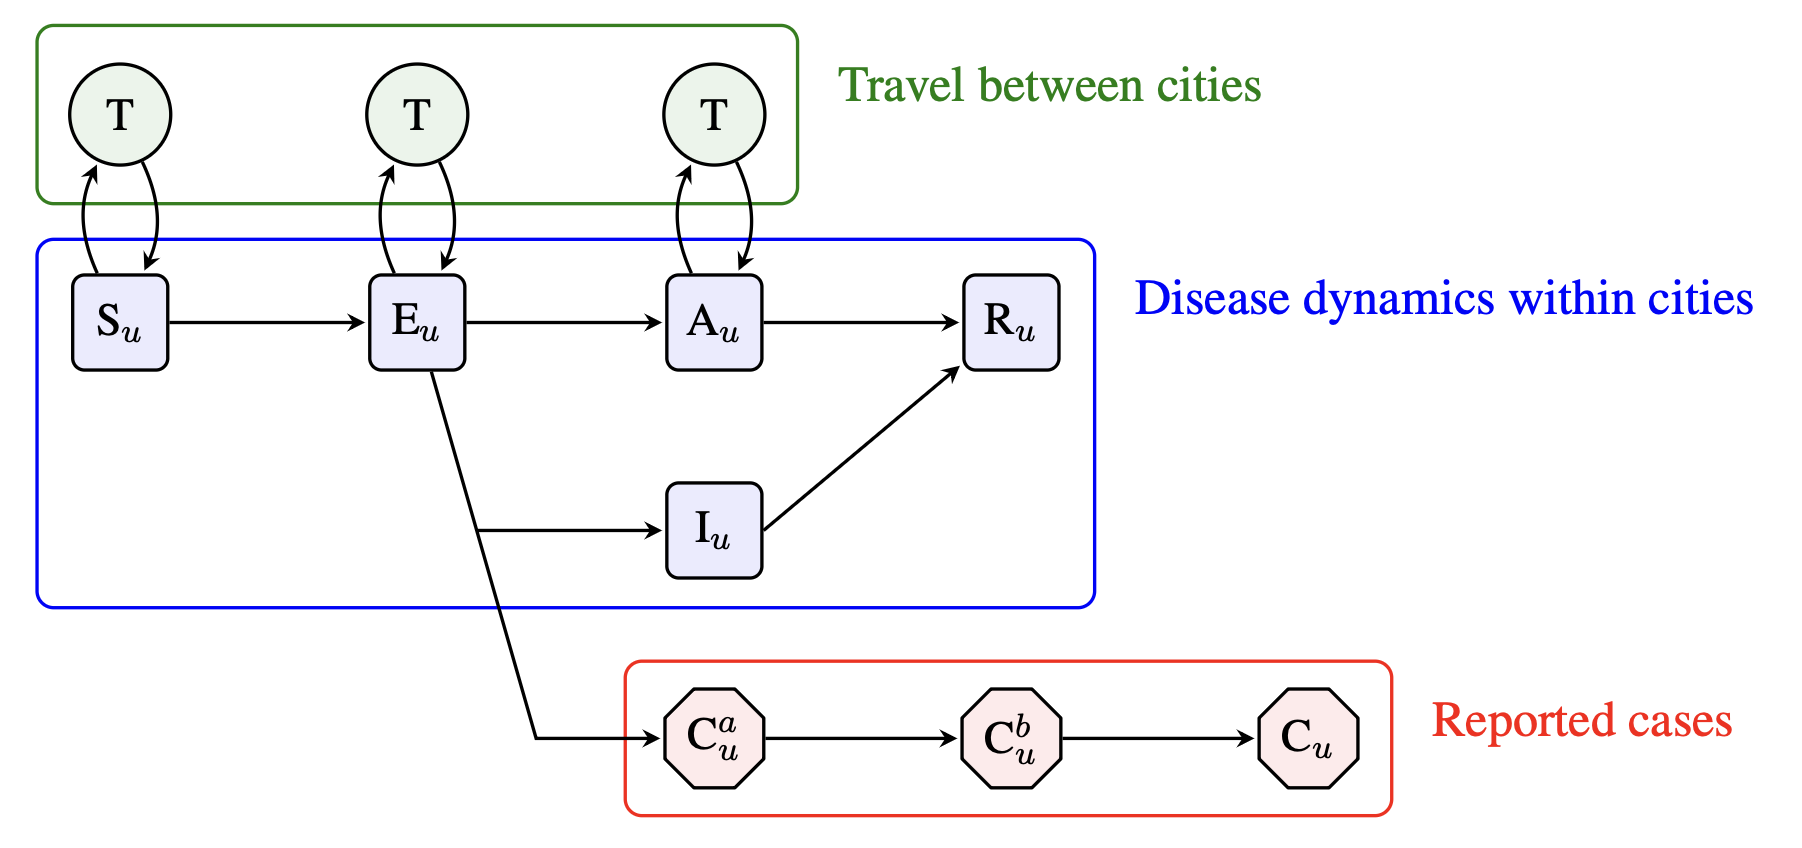
\includegraphics[height=5cm]{seair.png}
    \end{center}

\end{center}
\bi
\item 
  Reportably infectious individuals, $\mathrm{I}_u$ for city $u$, are included in the delayed reporting compartment, $\mathrm{C^a_u}$.
  \item 
An individual arriving at $\mathrm{C}_u$ is a case report for city $u$.
\item
  Individuals in $\mathrm{A}_u$ are not reportable and transmit at a reduced rate.
  \item 
Travel occurs to and from $\mathrm{T}$, based on 2018 data from Tencent.
%\item Many models have been proposed. We want a framework to implement and evaluate various scientific hypotheses.
\ei

\end{frame}

\begin{frame}{Log-likelihood values for six models}

  \resizebox{12cm}{!}{
\begin{tabular}{c|rr|l}
 & loglik & df & description
\\
\hline
$M_1$ &
  $-\infty$ & 10 &
  SEAIR model, parameter values and mobility of Li et al (2020)
\\
$M_2$ &  -14240.5 & 10 &
  Adjusted mobility and measurement in $M_1$
\\
$M_3$ &
 -11257.9  & 374 &
  Independent identically distributed negative binomial
\\
$M_4$ &
 -10825.3 & 375 &
  Autoregressive negative binomial
\\
$M_5$ &
  -9088.2&
  12 &
  Adding overdispersed dynamics to $M_2$ and refitting
\\
$M_6$ &
  -9116.5&
  10 &
  Latent and infectious periods unchanged by lockdown in $M_5$
\\

\hline
\end{tabular}
}

  \vspace{10mm}
  
Model comparisons by log-likelihood. The degrees of freedom (df) is the number of estimated parameters. 
  

\end{frame}

\begin{frame}{Data analysis progression}
  \bi
\item Some data errors meant that the original data was incompatible with the model.
\item Tracked down by assessing conditional log-likelihood for each unit and each time.
\item Even then, the likelihood was poor compared to non-mechanistic benchmarks. Including over-dispersion fixed that.
\item Some weak identifiability remained. extra assumptions can lead to plausible parameter estimates without much loss of model fit.
\item Mild outliers remain, e.g., Wuhan on day 18.  
  \ei

\end{frame}

\begin{frame}
  \begin{center}
    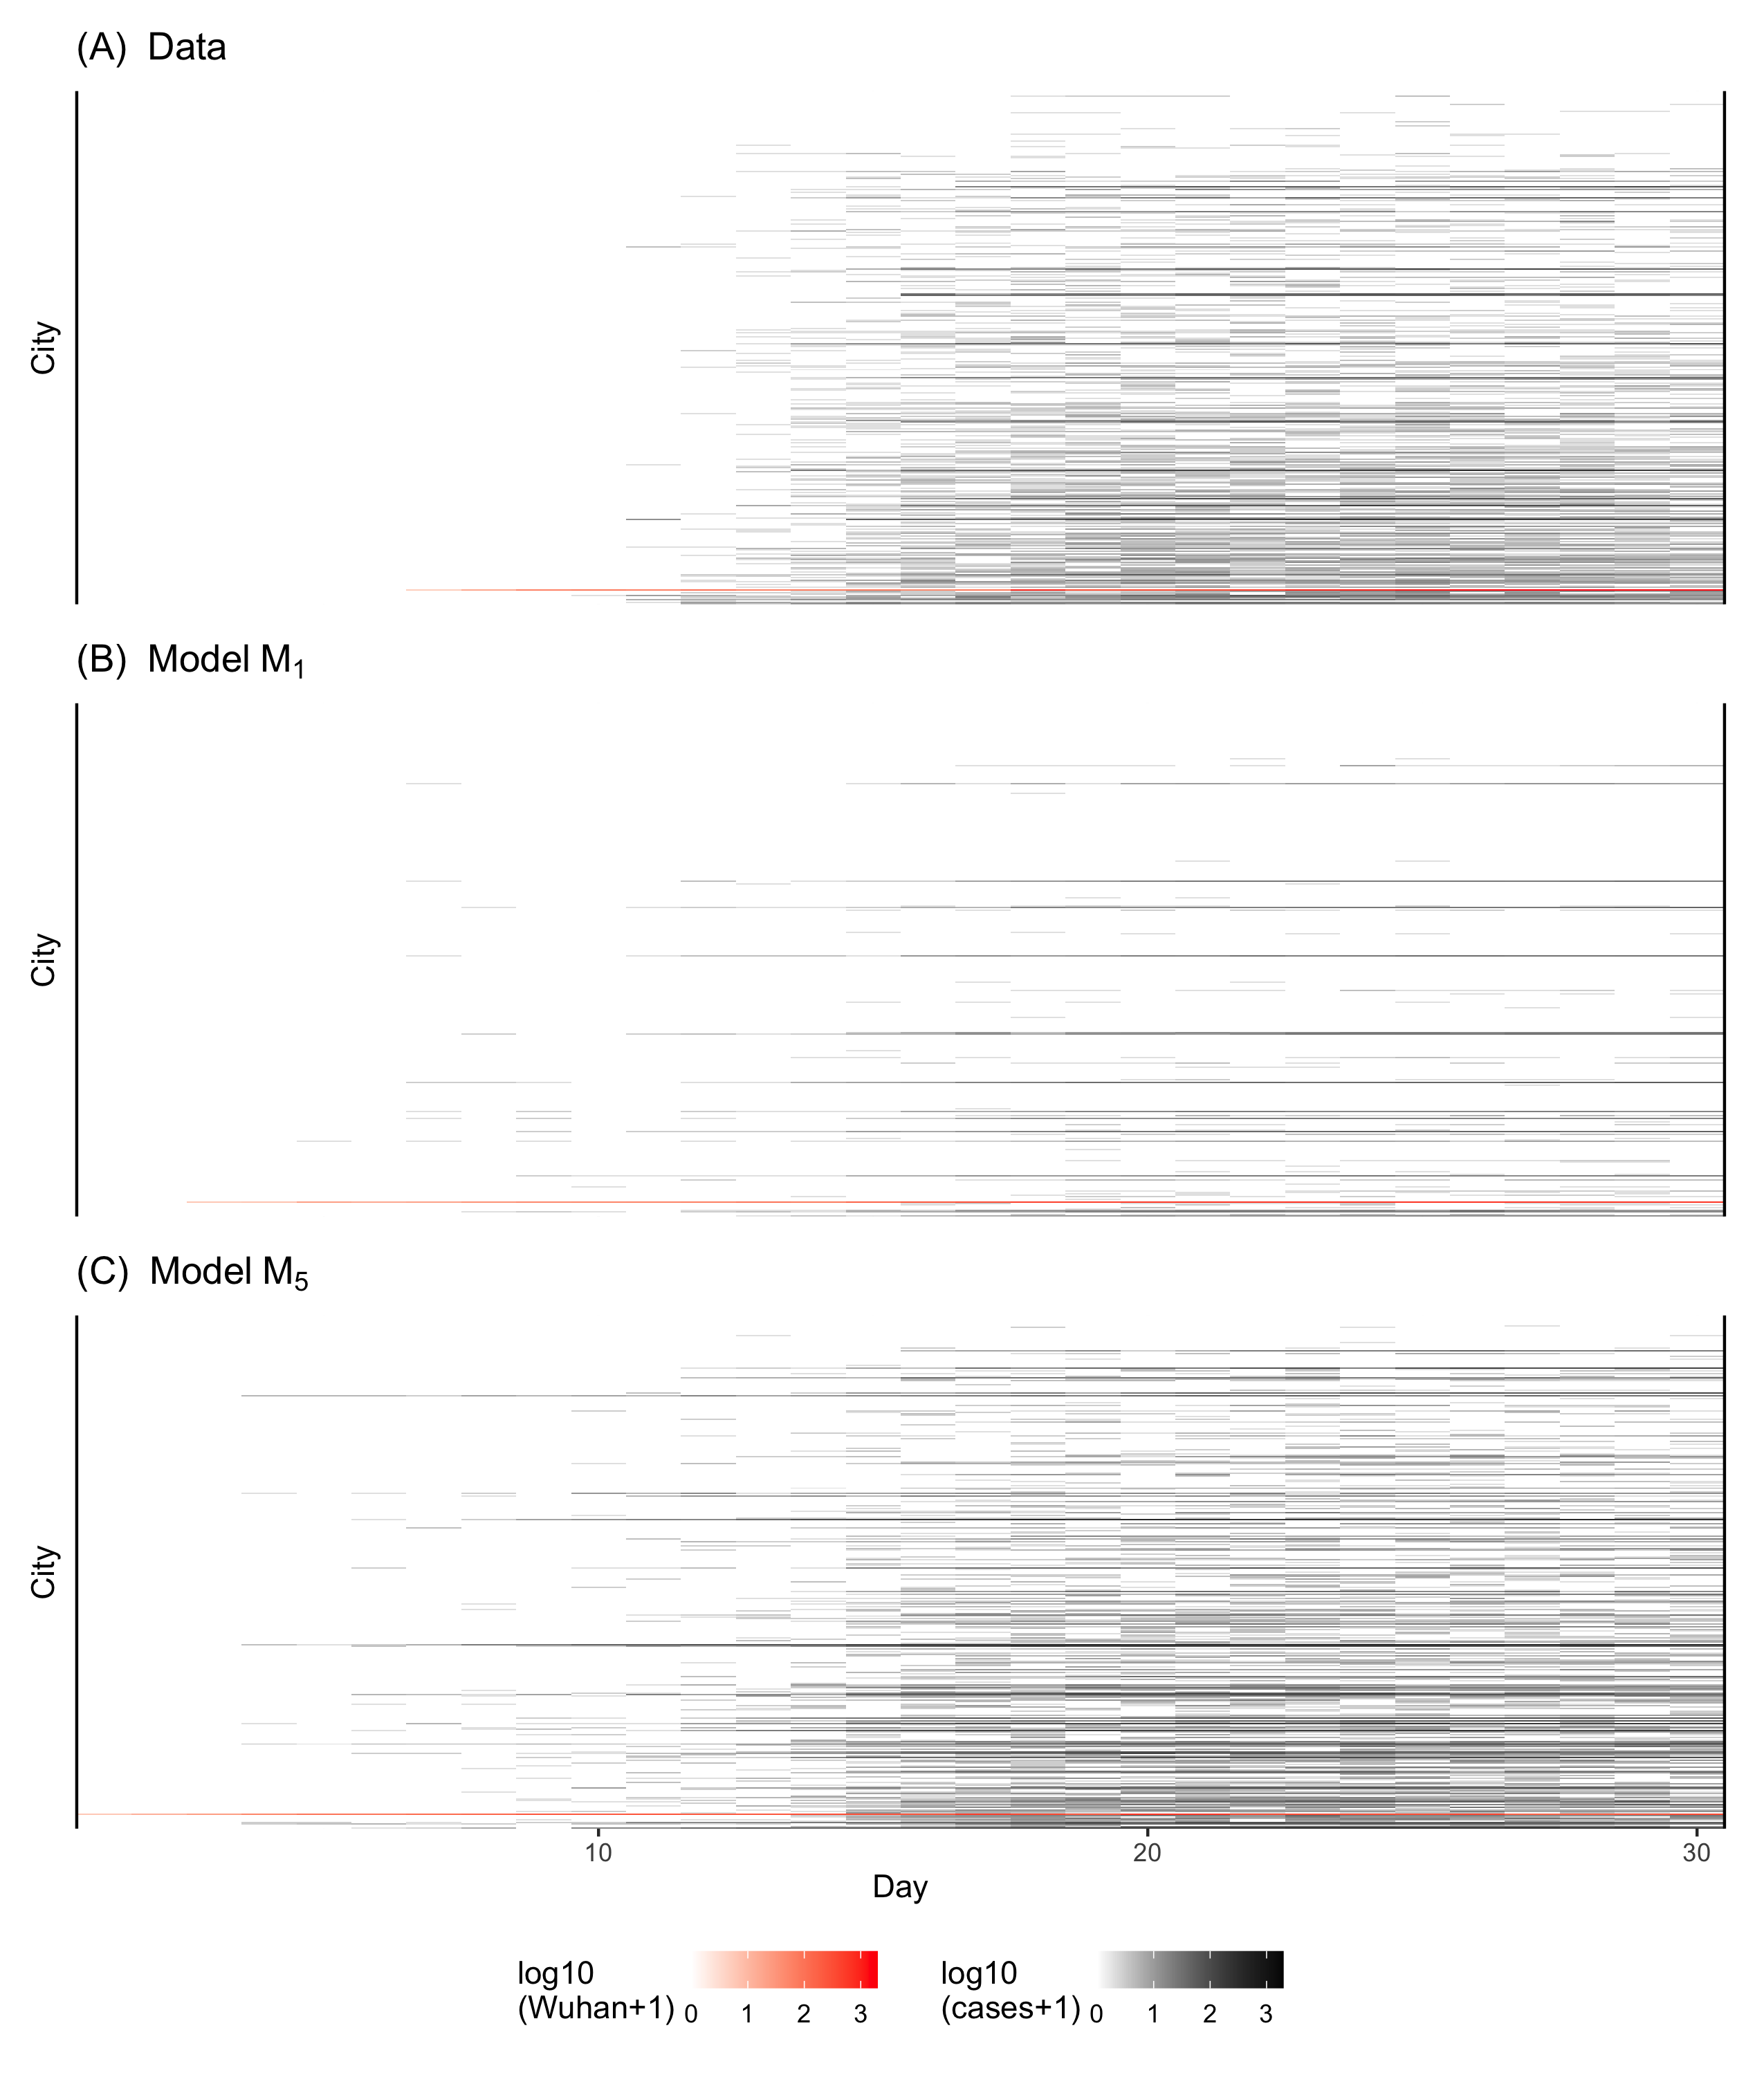
\includegraphics[height=9.5cm]{covid/panel_plot-1.png}
    \end{center}
\end{frame}


\begin{frame}
 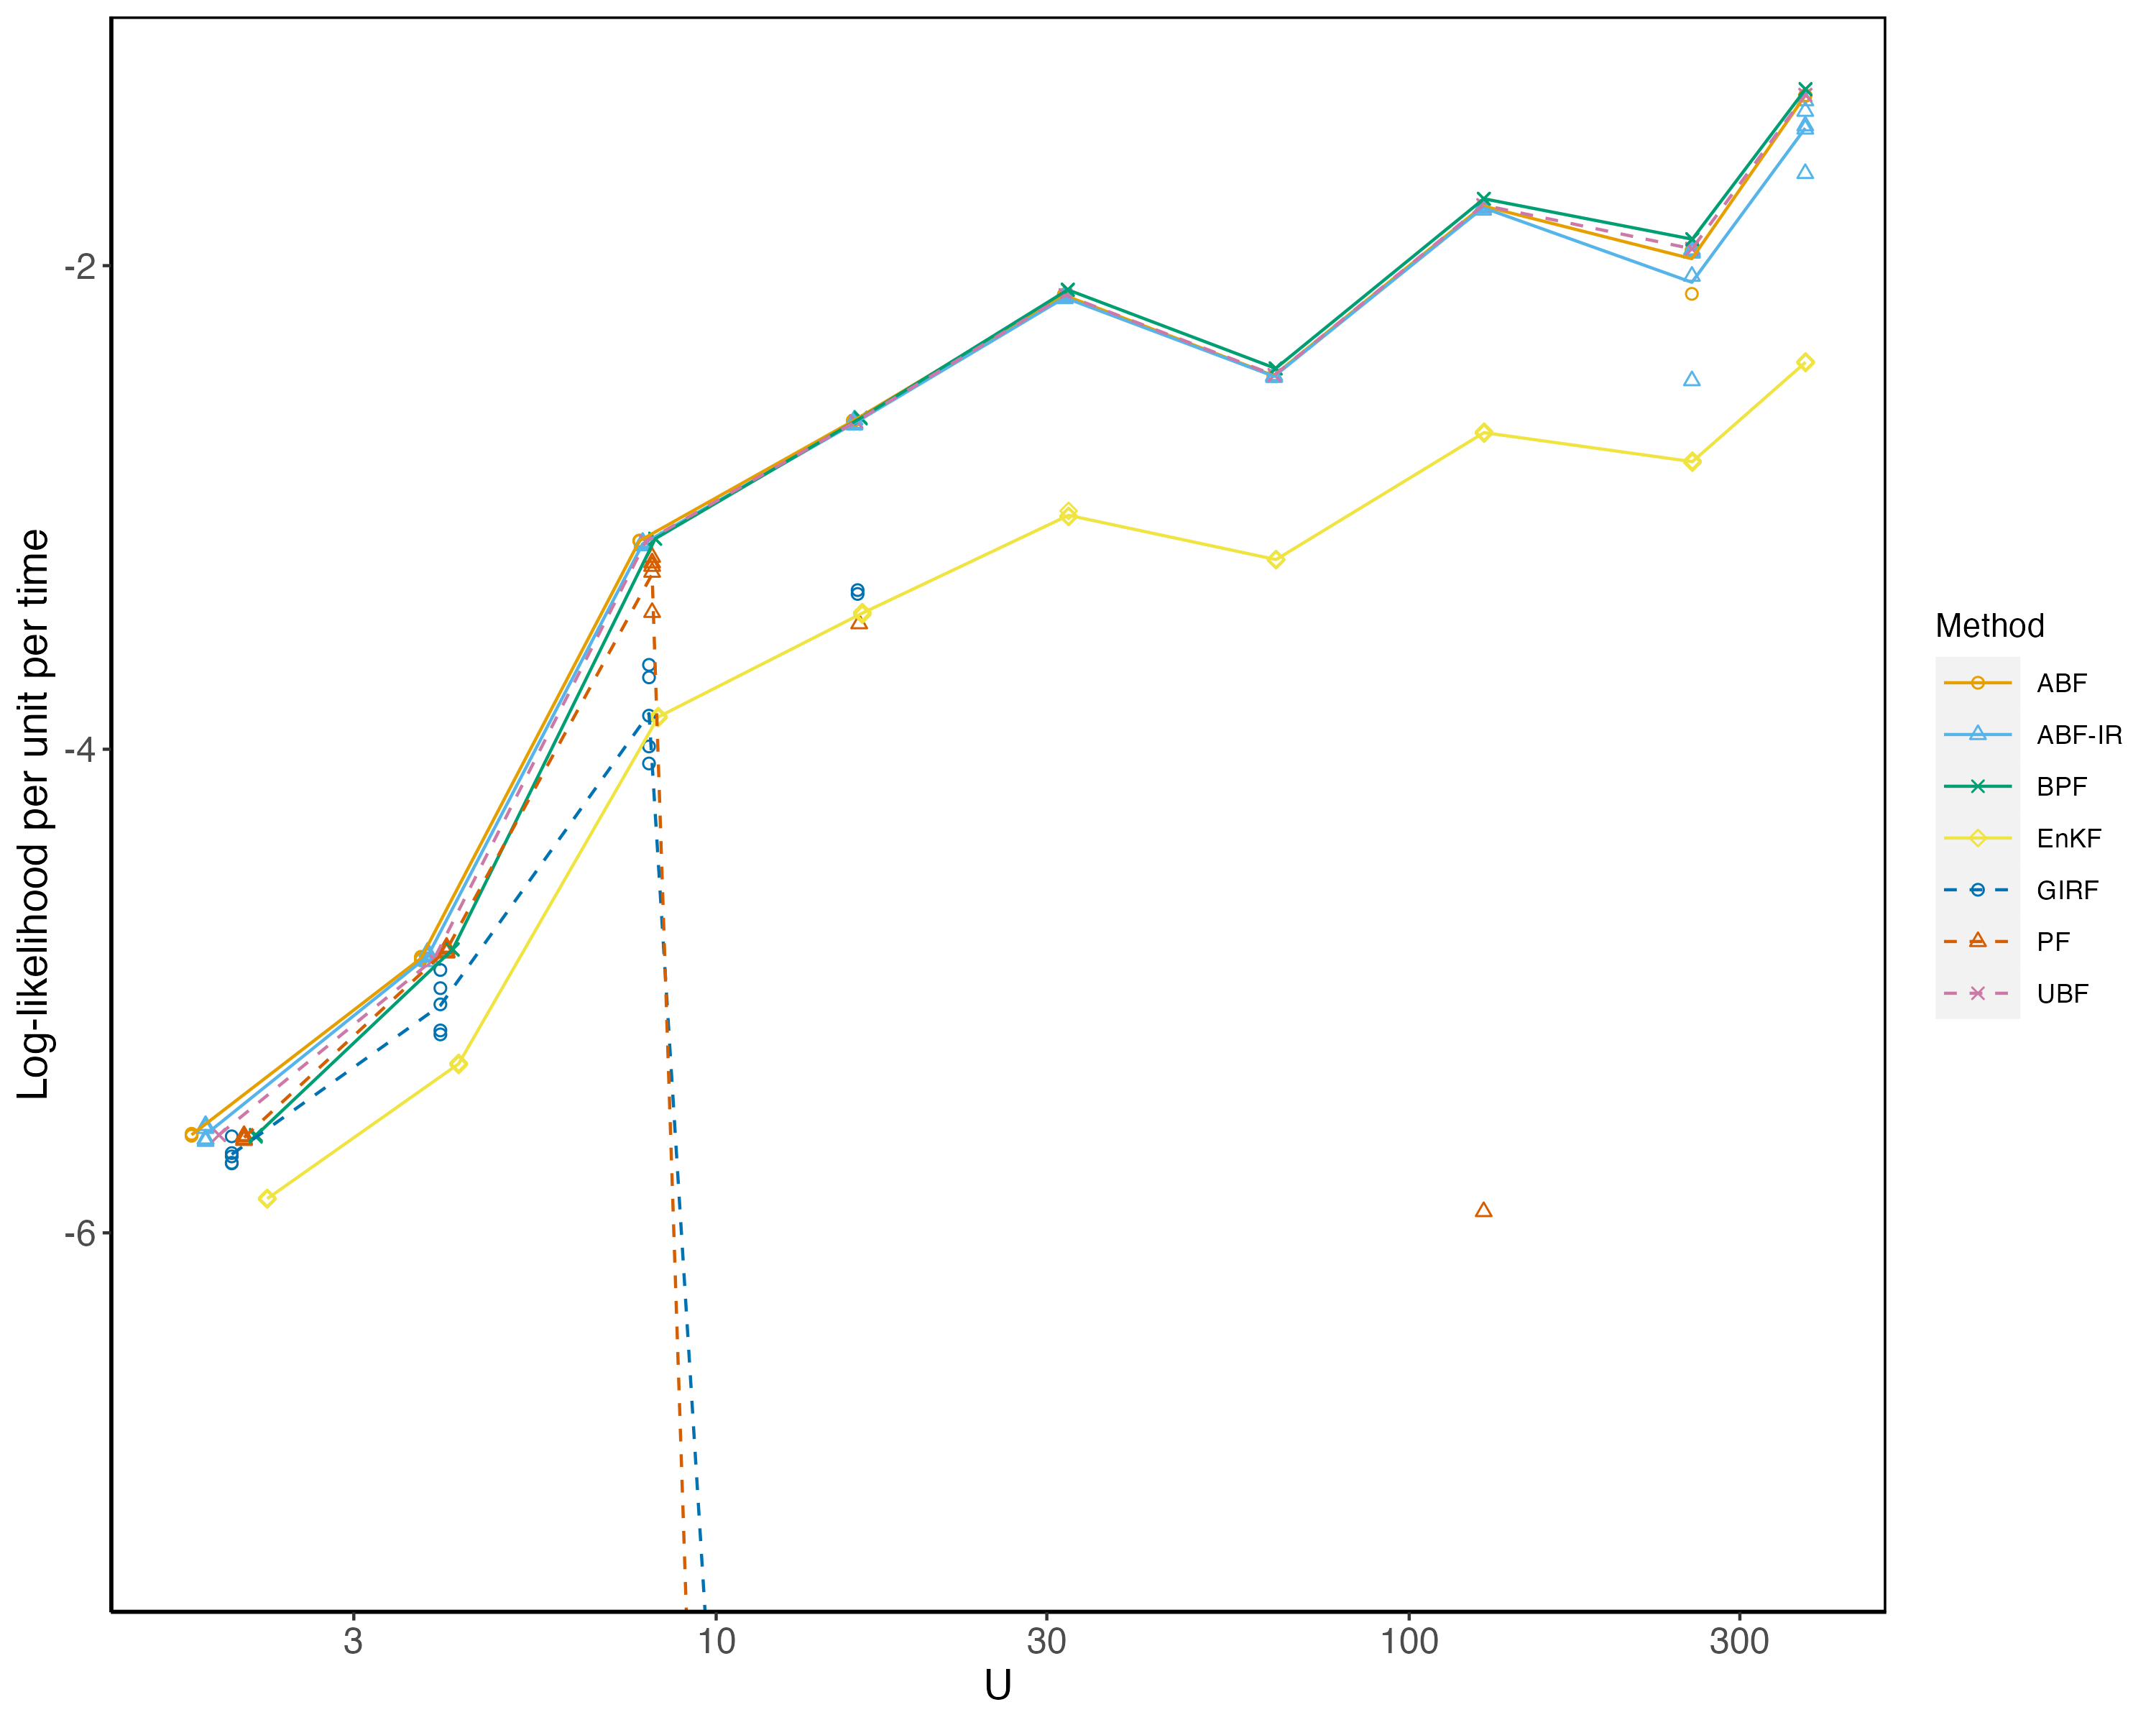
\includegraphics[width=10cm]{covid/filter_tests10.png}

  \begin{itemize}
\item BPF is the best available filter for this COVID model.
\item Similar results hold for other models (Ionides et al, {\it JASA}, 2023).
  \end{itemize}
  
\end{frame}

\begin{frame}{More on the block particle filter (BPF)}

\bi
\item BPF also worked quickly, easily and reliably on a measles metapopulation, as well as various toy benchmark problems (Ionides et al, {\it JASA}, 2023).

        \vspace{2mm}

\item BPF has theoretical support in some situations (Rebeschini \& Van Handel, {\it Annals of Applied Probability}, 2015).

        \vspace{2mm}

      \item This motivated us to develop an iterated BPF (IBPF) for parameter estimation.
        
        \vspace{2mm}

      \item IBPF has theoretical guarantees similar to BPF (Ning \& Ionides, {\it JMLR}, 2023).
        
        \vspace{2mm}

        
\item BPF was independently proposed as the ``factored particle filter'' by Ng et al (2002).

\ei

\end{frame}

\begin{frame}{Particle filter (PF)}

  \begin{columns}
    \begin{column}{0.48\linewidth}
      \begin{center}
      {\bf \textcolor{blue}{Evolutionary analogy}}

      \vspace{5mm}
      
      {\bf Mutation}

      $\downarrow$

      {\bf Fitness}

      $\downarrow$

      {\bf Natural selection}
      
      \end{center}
    \end{column}
     \begin{column}{0.48\linewidth}
      \begin{center}
      {\bf \textcolor{blue}{Particle filter algorithm}}

      \vspace{5mm}
      
      {\bf Predict: stochastic dynamics}

      $\downarrow$

      {\bf Measurement: weight}

      $\downarrow$

      {\bf Filter: resample}
      \end{center}
    \end{column}
  \end{columns}

  \vspace{15mm}
  
    \begin{myitemize}
  \item PF is an evolutionary algorithm with good mathematical properties: an unbiased likelihood estimate and consistent latent state distribution.
  \end{myitemize}

\end{frame}
  
\begin{frame}{Block particle filter (BPF)}

  \begin{myitemize}
    \item Blocks are a partition of the metapopulation units.
    \item For measles, we use each city as a block.
  \end{myitemize}
  
  \begin{columns}
    \begin{column}{0.48\linewidth}
      \begin{center}
      {\bf \textcolor{blue}{Evolutionary analogy}}

      \vspace{5mm}
      
      {\bf Mutation}

      $\downarrow$

      {\bf Fitness\\
      for each chromosome}

      $\downarrow$

      {\bf Natural selection\\
      for each chromosome}

      $\downarrow$

      {\bf Recombine chromosomes}
      
      \end{center}
    \end{column}
     \begin{column}{0.48\linewidth}
      \begin{center}
      {\bf \textcolor{blue}{Block particle filter}}

      \vspace{5mm}
      
      {\bf Predict: stochastic dynamics}

      $\downarrow$

      {\bf Measurement: weight\\
      for each block}

      $\downarrow$

      {\bf Filter: resample\\
      for each block}

      $\downarrow$

      {\bf Recombine blocks}
      \end{center}
    \end{column}
  \end{columns}

  \vspace{5mm}
  
    \begin{myitemize}
    \item Blocks are segments of the full state which can be reassorted between particles at the resampling step.

\end{myitemize}

\end{frame}


\begin{frame}{Comments on the Ensemble Kalman Filter (EnKF)}

  \begin{itemize}
  \item EnKF is more dependent on approximate Gaussianity than is sometimes supposed.

    \vspace{2mm}
    
  \item The Gaussian-inspired update rule is similar to the extended Kalman filter (EKF), which has largely been superseded by particle filter methods for low-dimensional nonlinear biological dynamics.

    \vspace{2mm}
    
\item Simple systems can defeat EnKF: the linear Gaussian update is helpless when data inform the conditional variance rather than the conditional mean.

  \vspace{2mm}
  
    \item Big systems need computationally tractable analysis. EnKF may sometimes be the best solution available, but be aware of its limitations.

  \end{itemize}

\end{frame}


\begin{frame}{An iterated block particle filter for parameter estimation}


  \begin{center}
    
%  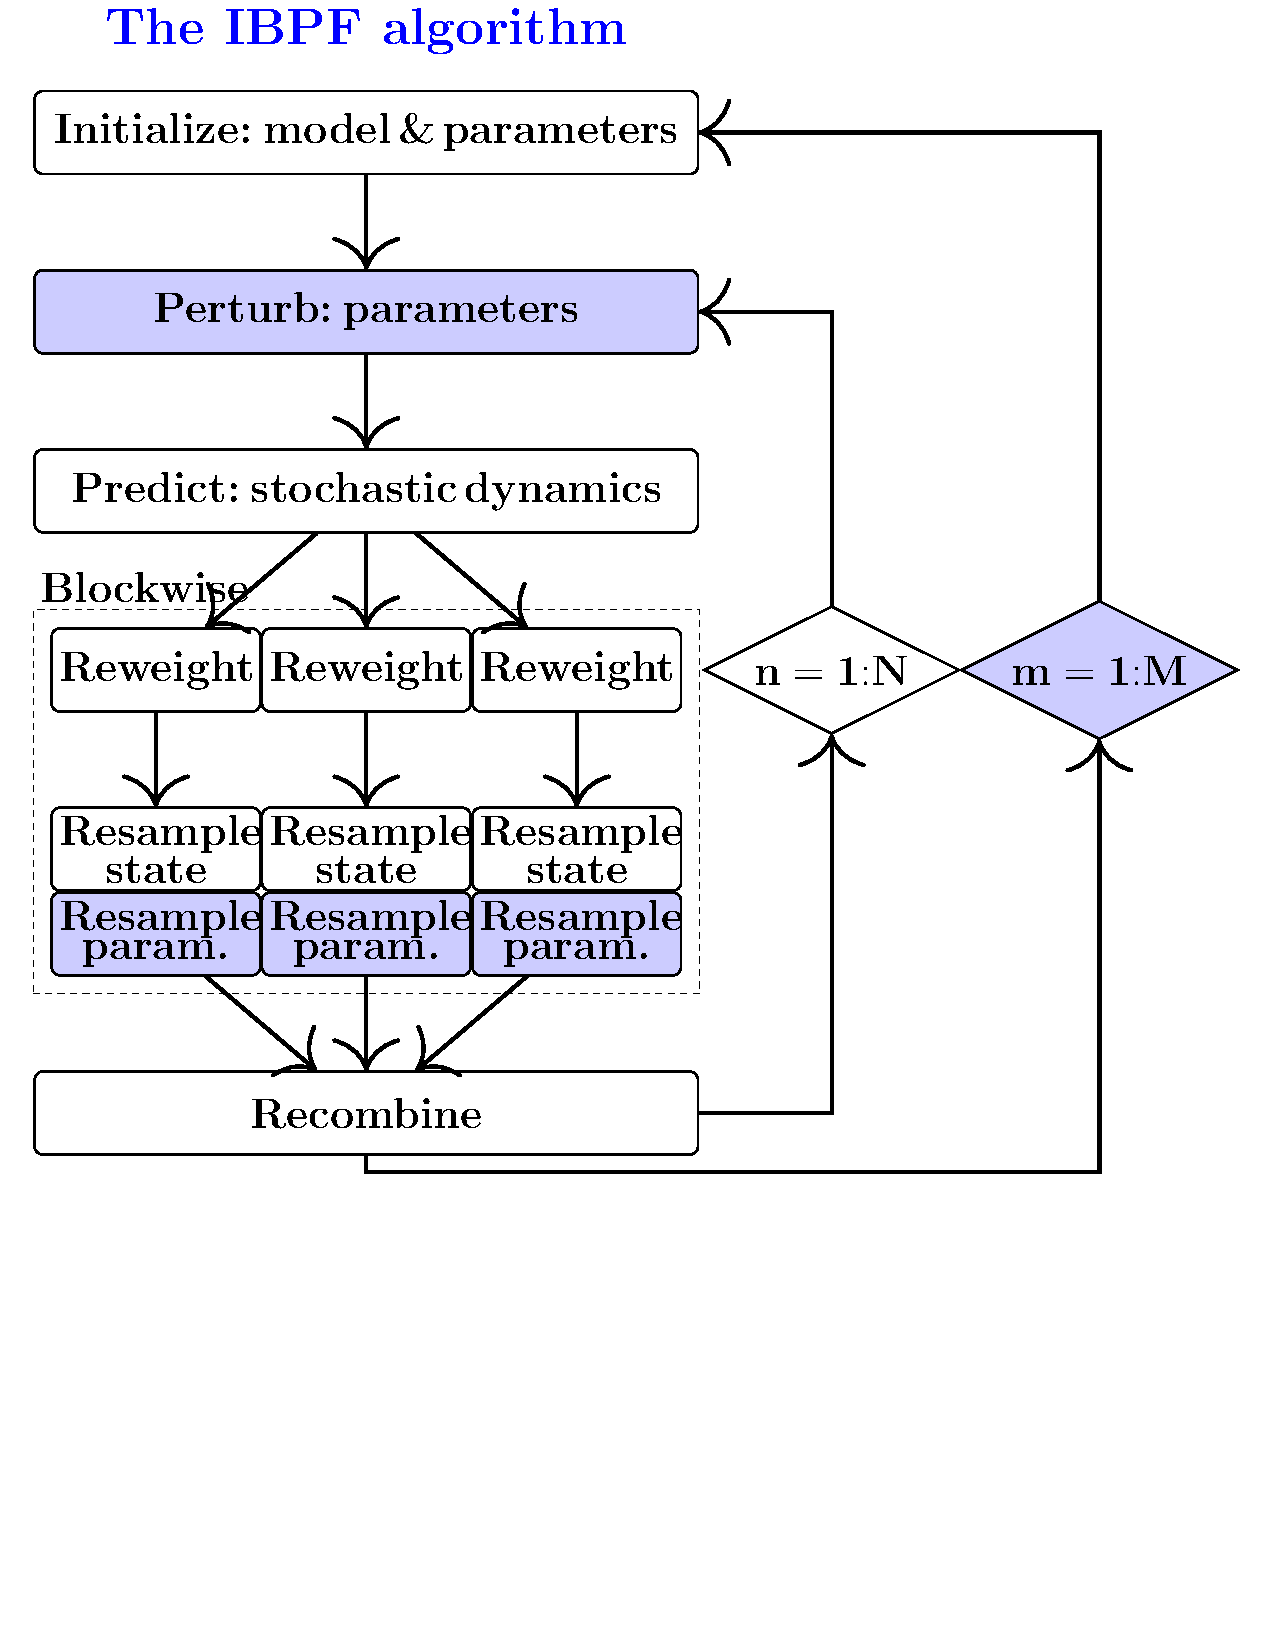
\includegraphics[trim={0 0 0 10mm},clip,width=9cm]{IBPF_workflow.pdf}
  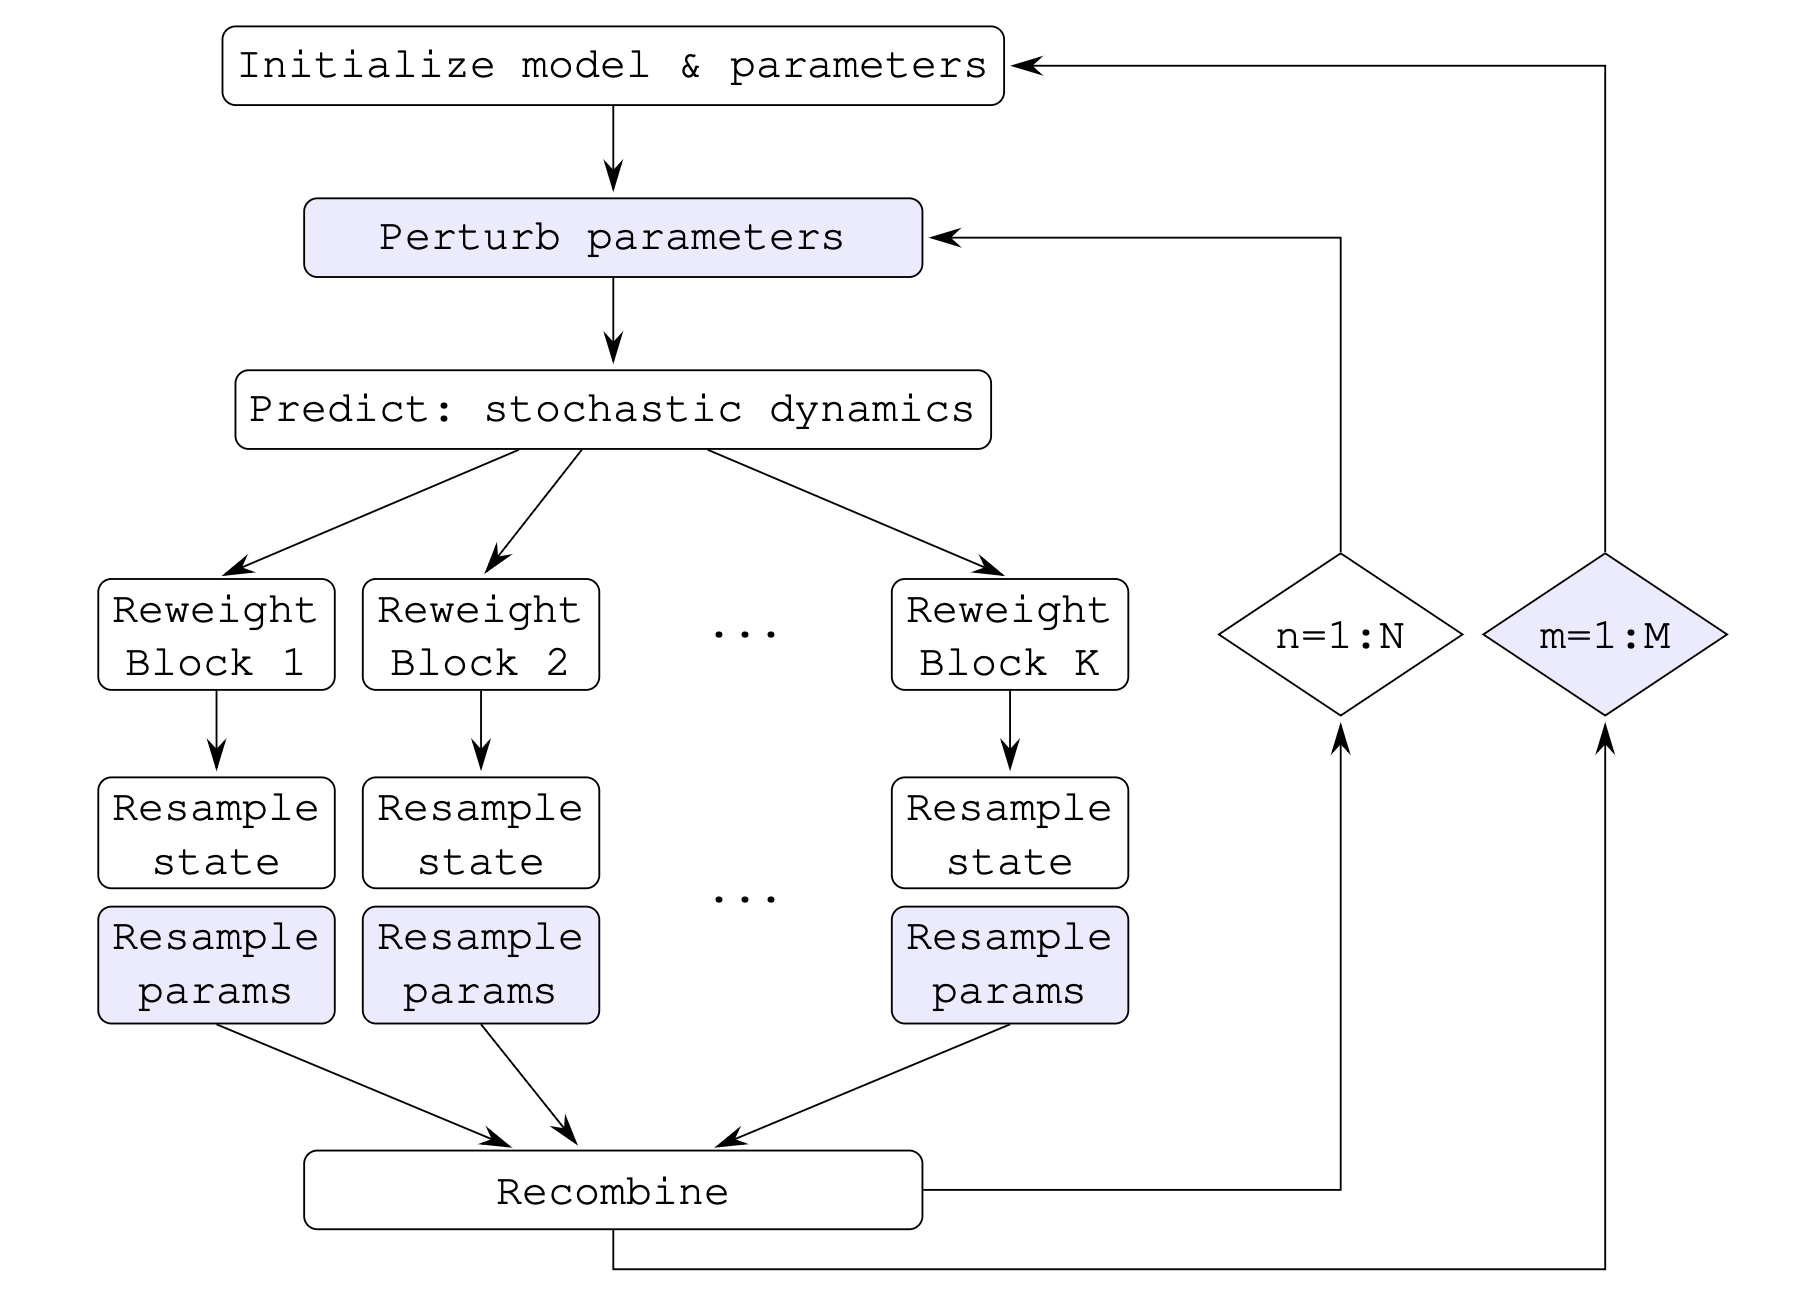
\includegraphics[width=11cm]{ibpf.png}


  \end{center}
  
\end{frame}

\begin{frame}{Practical inference using IBPF}
  \begin{enumerate}
  \item Monte Carlo adjusted profile likelihood \citep{ionides17profile} obtains confidence intervals that accommodate Monte Carlo error.

  \item Comparing the log-likelihood with an autoregressive model (or other simple statistical model) provides a check of model fit.

  \item Comparing the block log-likelihood against the benchmark provides insight into problematic units.

    \item Comparing the conditional log-likelihood for each observation against the benchmark helps to identify outliers. 

    \item Two recent case studies (Wheeler et al, 2023; Li et al, 2023) demonstrate data analysis using IBPF. Code and data are provided via R packages extending \code{spatPomp}.
      
  \end{enumerate}
  
  \end{frame}

\begin{frame}{Filtering $U$ units of a coupled measles SEIR model}

\vspace{-1mm}

\begin{center}
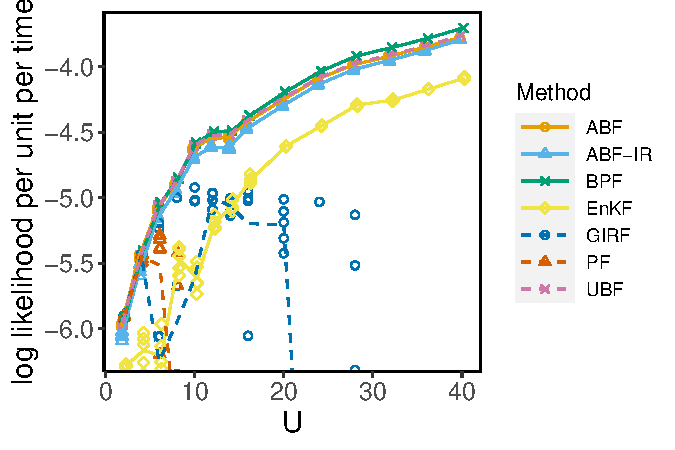
\includegraphics[width=10cm]{mscale_loglik_plot-1.pdf}


\end{center}

\vspace{-4mm}

Simulated data using a gravity model with geography, demography and transmssion parameters corresponding to UK pre-vaccination measles (Ionides et al, {JASA}, 2023).

%\end{center}

\end{frame}


\begin{frame}
\frametitle{Filtering $U$-dimensional correlated Brownian motion}

\vspace{-3mm}

\begin{center}
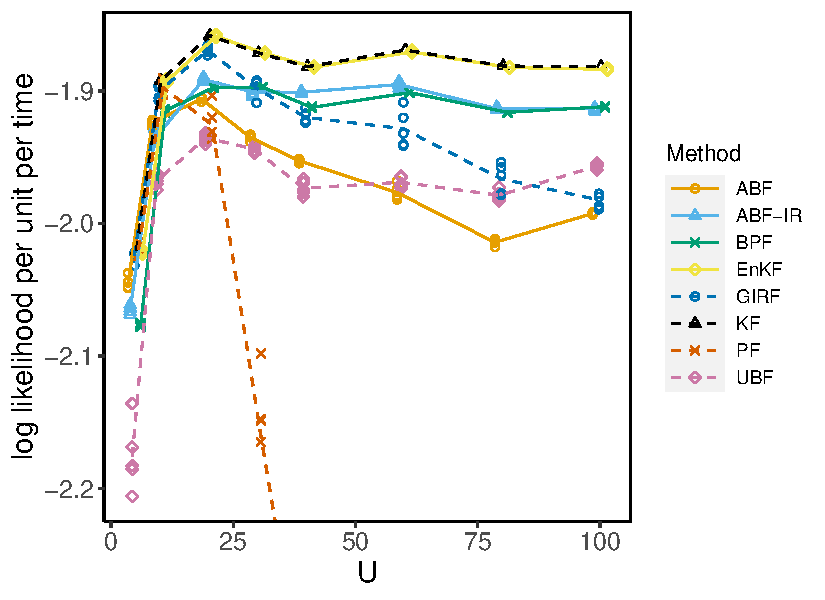
\includegraphics[width=10cm]{bm_alt_plot-1.pdf}

\vspace{-1mm}

$\cov\big(X_{\unit,\time}-X_{\unit,\time-1},X_{\altUnit,\time}-X_{\altUnit,\time-1}\big) \sim 0.4^{|\unit-\altUnit|}_{}$

\end{center}

\end{frame}

\begin{frame}
\frametitle{Filtering $U$ units of Lorenz 96 toy atmospheric model} 

\vspace{-3mm}

\begin{center}
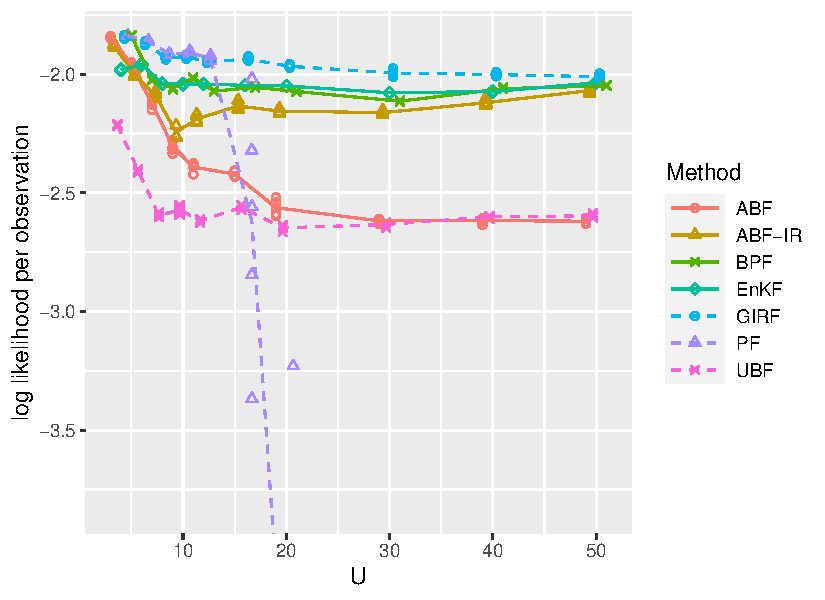
\includegraphics[width=10cm]{lz_loglik_plot-1.pdf}

\vspace{-1mm}

$dX_{\unit}(t) = \big \{  X_{\unit-1}(t) \big(X_{\unit+1}(t) - X_{\unit-2}(t)\big) - X_{\unit}(t) + F \big\} dt + \sigma \, dB_{\unit}(t)$

\end{center}

\end{frame}


\nocite{asfaw24,bjornstad01,breto19,grenfell04,he10,katzfuss19,ionides21,ionides24,lee20,li20,ng02,ning23-ibpf,park20,rebeschini15,wheeler24,li24}

\nocite{asfaw24tutorial}
\begin{frame}[allowframebreaks]
\frametitle{References}
\bibliographystyle{apalike}
\bibliography{bib}
\end{frame}

%%% extra material


\end{document}
